\documentclass[11pt,a4paper]{article}
\usepackage[utf8]{inputenc}
\usepackage[T1]{fontenc}
\usepackage{lmodern}
\usepackage[french]{babel}
\usepackage[margin=2.1cm]{geometry}
\usepackage{microtype}
\usepackage{amsmath,amssymb}
\usepackage{booktabs}
\usepackage{array}
\usepackage[table]{xcolor}
\usepackage{graphicx}
\usepackage{caption}
\usepackage{eurosym}
\usepackage[most]{tcolorbox}
\definecolor{navy}{HTML}{1F3864}
\definecolor{bluemid}{HTML}{2E5496}
\definecolor{lightblue}{HTML}{D6E0F0}
\captionsetup{font=small,labelfont={bf,color=navy},labelsep=period}
\graphicspath{{../figures/}}
\newtcolorbox{cle}[1][]{colback=lightblue!40,colframe=navy,boxrule=0.6pt,
  arc=2pt,left=8pt,right=8pt,top=6pt,bottom=6pt,#1}

\title{\vspace{-1.2cm}\color{navy}\bfseries La bande de modèle\\[2pt]
  \large Le troisième étage d'incertitude du SCR}
\author{Kélian Kaddouri}
\date{27 juillet 2026}

\begin{document}
\maketitle
\vspace{-0.9cm}

\begin{cle}
\textbf{La question.} \og{}Chaque modèle peut-il être remis en cause par une autre méthode~?\fg{}
Oui, sans exception. L'incertitude sur le SCR se cumule sur trois étages : \textbf{paramètre}
(bootstrap sur $\xi$), \textbf{identification} (bornes sur la direction $W$), et \textbf{modèle}
(le choix de la famille elle-même). On chiffre ce troisième étage, le plus souvent passé sous
silence.
\end{cle}

\medskip
\begin{center}
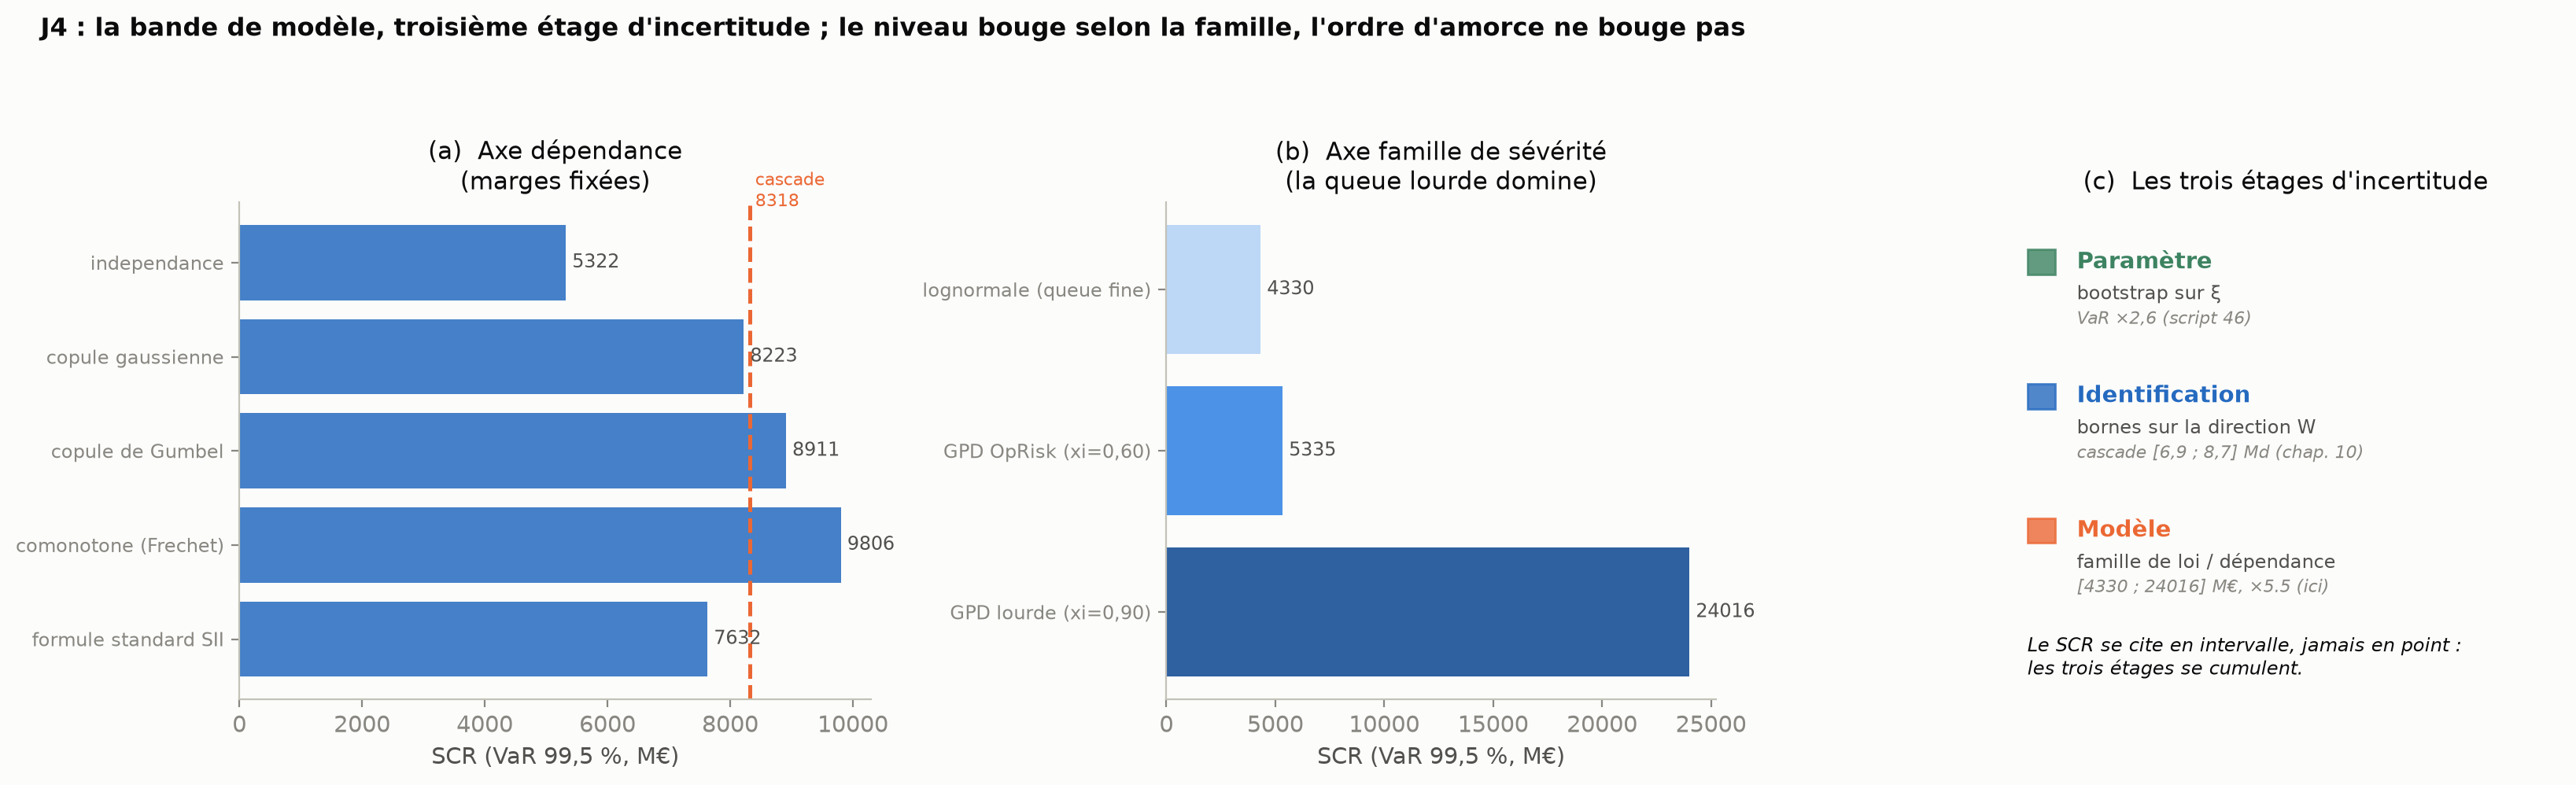
\includegraphics[width=\linewidth]{J4_bande_modele.png}
\captionof{figure}{\textbf{(a)} axe dépendance, à marges fixées : la cascade se place entre les
copules gaussienne et de Gumbel. \textbf{(b)} axe famille de queue : la queue lourde domine
l'incertitude. \textbf{(c)} les trois étages (paramètre, identification, modèle) se cumulent.}
\end{center}

\noindent\textbf{Axe dépendance} (marges par pilier fixées) : le SCR va de $5\,322$ M\euro{}
(indépendance) à $9\,806$ M\euro{} (comonotone, borne de Fréchet), soit un facteur $1{,}8$ ; la
formule standard Solvabilité~II et les copules gaussienne et de Gumbel se placent entre les
deux. Notre \textbf{cascade dirigée} ($8\,318$ M\euro) tombe dans cette bande, entre une
dépendance gaussienne et une dépendance de Gumbel : elle n'est ni extrême ni arbitraire.

\medskip
\noindent\textbf{Axe famille de queue} (agrégation en indépendance) : d'une lognormale
($4\,330$ M\euro) à une GPD à queue lourde $\xi=0{,}90$ ($24\,016$ M\euro), un facteur $5{,}5$.
C'est le choix de la loi de queue qui domine, de loin, l'incertitude de modèle --- et c'est
pourquoi le plafond de réassurance ($40$ M\euro) est un levier distinct, qui ramène la famille
lourde à $495$ M\euro : une réponse au risque de queue, non le risque lui-même.

\begin{cle}
\textbf{Le niveau bouge, l'ordre ne bouge pas.} Fréquence (Poisson, Hawkes, Cox), sévérité
(lognormale, splicing, EVT bayésienne), dépendance (copules, réseaux), mesure (TVaR, spectrale,
robuste), agrégation (formule standard, Panjer) : on ne prétend pas détenir \emph{la} méthode.
On a testé les concurrents sérieux, on \textbf{borne} l'effet du choix, et surtout l'ordre
d'amorce des piliers ($P1>P4>P2>P3>P5$) est \textbf{invariant} à la famille. Le niveau est
illustratif, l'ordre résiste : la thèse du mémoire, chiffrée sur un troisième axe.
\end{cle}

\smallskip
\noindent\footnotesize\textcolor{navy}{\textbf{Source.}} Script
\texttt{1\_fondations/48\_bande\_modele.py}, figure \texttt{J4\_bande\_modele.png}.

\end{document}
